\section{Modificaciones de la arquitectura y desarrollo}
\subsection{Entrenamiento}
Script de entrenamiento, dataloader, todas las cosas que se han hecho para acelerar el entrenamiento. Hablar de las horas de entrenamiento? Puede que se mezclen cosas con el apartado de metodología?
\subsection{Reducción de tamaño de la entrada}
\subsection{Número de cabezas}
Hablar del cambio en el número de cabezas
\subsection{Capas de atención eficiente}
Cambio de las capas, hacer una gráfica midiendo en función del tamaño de la cadena la velocidad en la que pasa por una de estas capas? Puede ser interesante. (Sería para imágenes mayores)
\subsection{Cambio en los hooks del transformer y eliminación de las capas de atención posteriores}
Lorem
\begin{figure}[H]
\centering
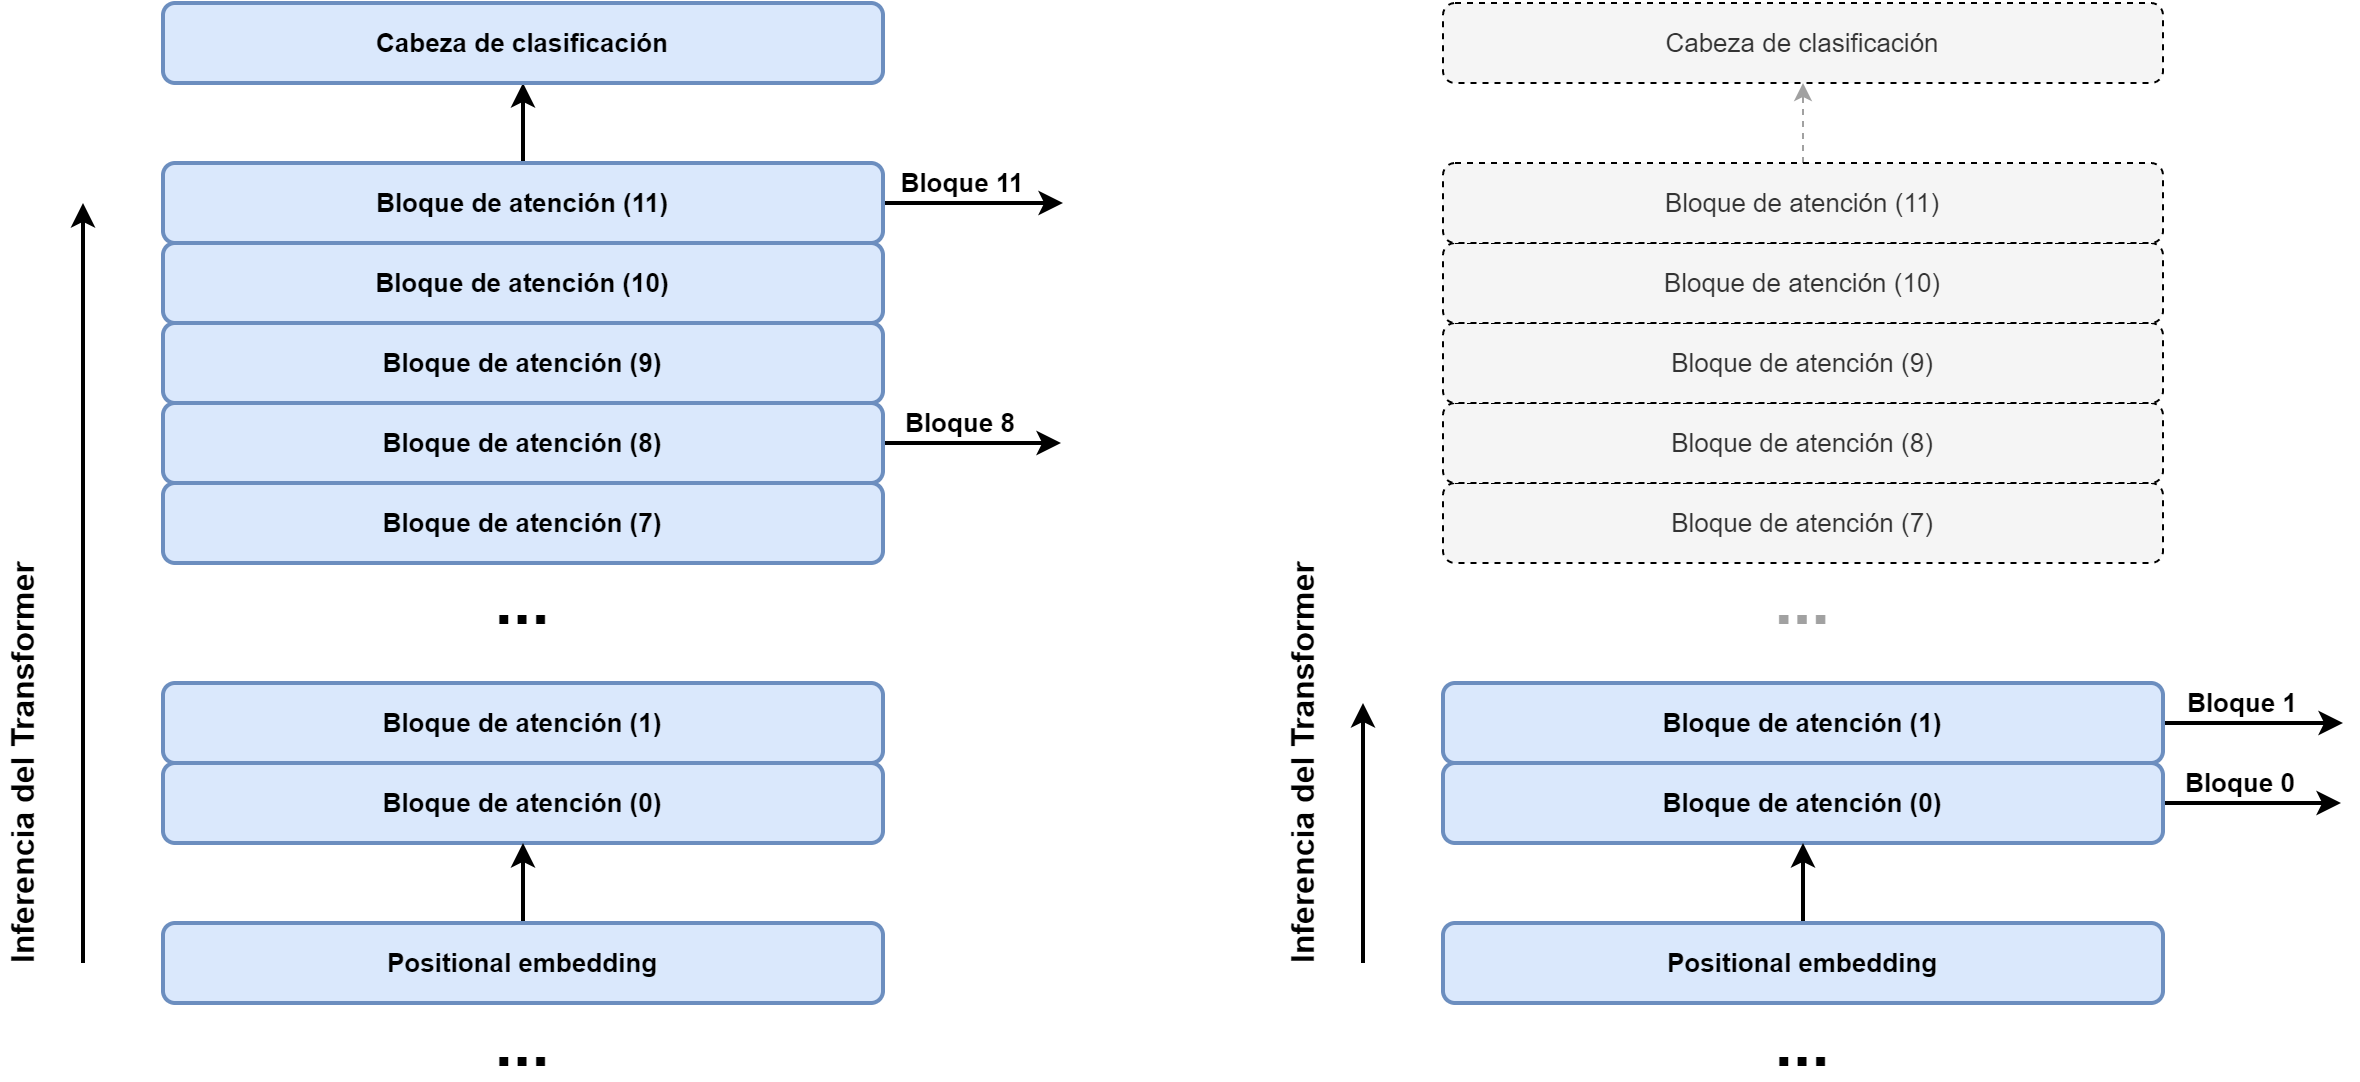
\includegraphics[width=\textwidth]{imagenes/DPT-cambio-bloques-transformer.png}
\caption{Cambio en el número de bloques de atención.}
\label{fig:attention_block_num}
\end{figure}

\begin{figure}[H]
\centering
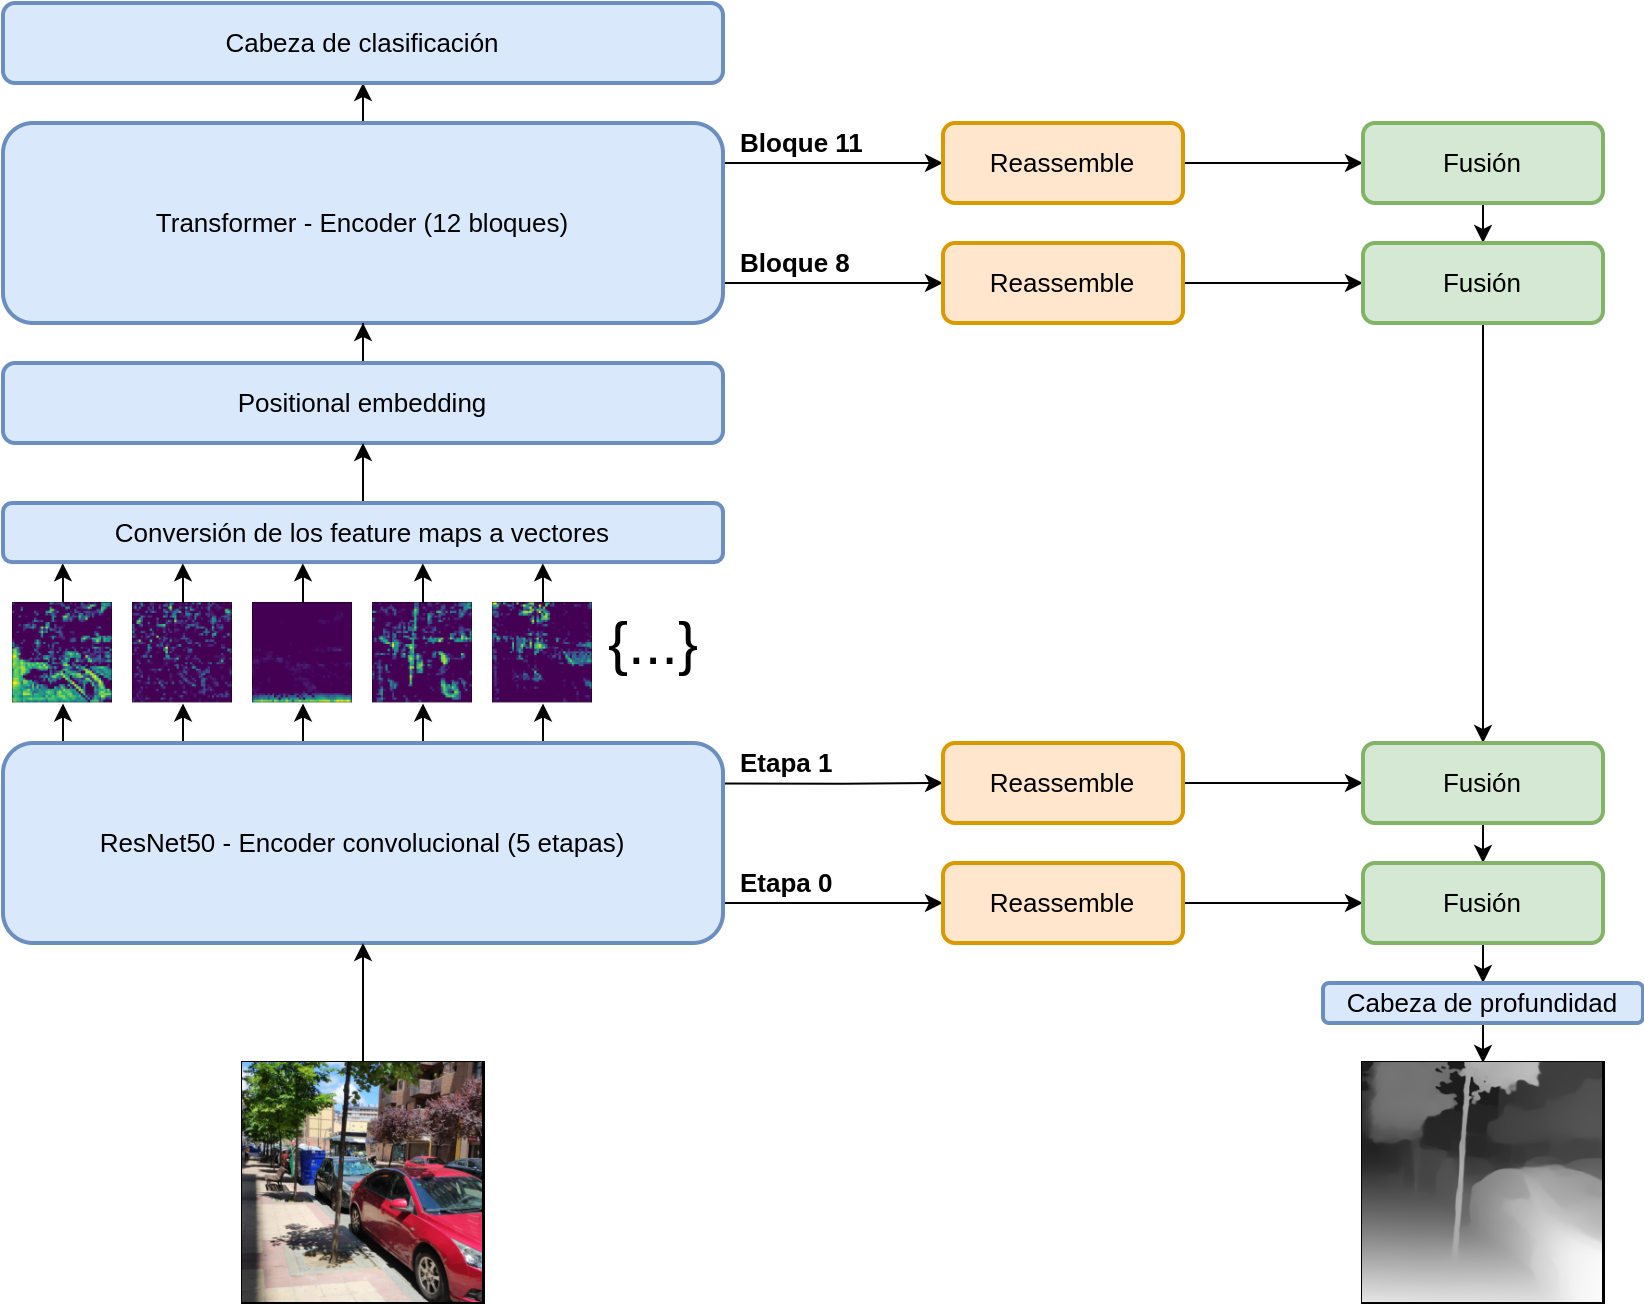
\includegraphics[width=\textwidth]{imagenes/DPT-general.png}
\caption{Arquitectura general DPT.}
\label{fig:dpt-general}
\end{figure}

\begin{figure}[H]
\centering
\includegraphics[width=\textwidth]{imagenes/DPT-modificado-general.png}
\caption{Arquitectura general DPT tras las modificaciones.}
\label{fig:dpt-mod-general}
\end{figure}

\subsection{Cambio del backbone convolucional}
Lorem


% En los resultados hablar de la distribución de los pesos antes y después de convertir el modelo si es pertinente, hacer una especie de estudio de ablación si se puede entrenar modelos, etc. Puede estar interesante quitar cabezas de atención, quitar bloques de atención, ver como afecta al tamaño dle modelo, su rendimiento (velocidad y métricas)...

\clearpage